%\documentclass[journal=jacsat]{achemso}

\documentclass[aps,prb,twocolumn,amsmath,amssymb,superscriptaddress,longbibliography]{revtex4-1}

%\documentclass[preprint,showpacs,preprintnumbers,amsmath,amssymb]{revtex4-1}
%\documentclass[twocolumn,showpacs,preprintnumbers,amsmath,amssymb]{revtex4}
% Some other (several out of many) possibilities
%\documentclass[preprint,aps]{revtex4}
%\documentclass[preprint,aps,draft]{revtex4}
%\documentclass[prb,amsmath,amssymb]{revtex4}% Physical Review B

\usepackage{tikz} %for adding axes labels to figures
\usepackage{graphicx}% Include figure files
\usepackage{epstopdf} %convert graphics
\usepackage{dcolumn}% Align table columns on decimal point
\usepackage{bm}% bold math
\usepackage{amsmath}% bold math
\usepackage{color}
\usepackage{booktabs}
%\usepackage[normalem]{ulem}
%\nofiles
\usetikzlibrary{positioning}

%shortcuts for sets of numbers
\newcommand{\Ns}{\mathbb{N}^{*}}
\newcommand{\N}{\mathbb{N}}
\newcommand{\Z}{\mathbb{Z}}
\newcommand{\Zs}{\mathbb{Z}^{*}}
\newcommand{\R}{\mathbb{R}}
\newcommand{\Rs}{\mathbb{R}^{*}}
\newcommand{\C}{\mathbb{C}}
\newcommand{\Cs}{\mathbb{C}^{*}}

\newcommand{\angstrom}{\text{\normalfont\AA}}
\newcommand\tab[1][1cm]{\hspace*{#1}} %tab shortcut

\begin{document}

\title{
%Using absolutely localized molecular orbitals for deeper physical insight into the nature of chemical bonding and linear-scaling calculations for condensed phase [binary] materials 
%Localized electrons (orbitals) in materials modeling
Comparative study of empirical force-field and DFT models of amorphous $\text{TiO}_2$ nanoparticles
%Absolutely localized orbitals for density functional theory modeling of [binary] materials
}

\author{Nicolas Gastellu}
%\author{Yifei Shi}
\author{Rustam Z. Khaliullin}
\email{rustam.khaliullin@mcgill.ca}
\affiliation{Department of Chemistry, McGill University, 801 Sherbrooke St. West, Montreal, QC H3A 0B8, Canada}

\date{September 3, 2018}

\begin{abstract}

We calculate the energy of the conformations of amorphous titania nanoparticles obtained in classical MD simulations at $T=300\,$K using the classical two-body Matsui-Akaogi (MA) potential and Kohn-Sham density functional theory (DFT) in the Perdew-Burke-Ernzerhof approximation. 
Comparative analysis of the energies shows the values obtained using the MAP formalism are only weakly correlated with those calculated with DFT. 
Remarkably we also found that a simple rutile nanocrystal (RZK: is this a nanocrystal? it is supposed to be perfect periodic lattice), for which the MA potential is expected to be well-parameterized, exhibited almost no correlation between the two sets of calculated energies. 
We discuss possible reasons for this discrepancy and examine implications of our results, chief among them is the suitability of the classical MA potential for amorphous titania nanoparticles.


\end{abstract}

\maketitle
 

\section*{Introduction} 

\tab Titania ($\text{TiO}_2$) has long been the subject of notable research interest due to its high chemical stability and interesting optical, dielectric, mechanical, and photocatalytic properties\cite{optical,thin-film,mechanical,photocatalytic}. 
While most works focus on $\text{TiO}_2$ in its most stable and common forms, which are all crystalline, a number of technological uses of this material rely on processing into film or powder form which both tend to be amorphous; further modification of the material is then needed to restore it to a certain level of crystalline order\cite{a2c,ab_initio}.
Dependence on this last step makes titania significantly more difficult and expensive to to use in industrial-scale applications, which has motivated researchers to study amorphous $\text{TiO}_2$ ($a-\text{TiO}_2$) in hope of being able to use in it cheaper, less processed forms\cite{useful1,useful2,useful3}. 
%As such, there is a need for a better understanding of amorphous $\text{TiO}_2$'s structure and properties ($a-\text{TiO}_2$) in order to utilise them to their full potential in novel technological applications, but also to ensure that our current modes of implemening $a-\text{TiO}_2$ in devices will not exhibit any unforeseen behaviour due to our poor understanding of the material's characteristics. 

\tab One of the defining traits of amorphous materials is their lack of long-range order, which makes their microstructure hard to study experimentally.
In spite of this, recent experimental studies have been successful in describing the local atomic structure of $a-\text{TiO}_2$ under different environments\cite{exptl1,exptl2,exptl3} by measuring structural properties such as the coordination number of bulk and surface Ti atoms and average bond lengths, using various types of X-ray absorption structure spectroscopy.
However, the most detailed investigations of amorphous titania's structure have been those combining experimental methods (e.g. X-ray absorbtion spectroscopy) with the computation modeling (notably reverse Monte-Carlo simulations)\cite{comp_exptl1,comp_exptl2,comp_exptl3}.
Our reliance on simulations to properly understand this material is a major research incentive for theoretical chemists to devise the adequate computational tools.

\tab While computational chemistry software employs a miscellany of procedures to generate results, one can distinguish two main approaches to running such calculations:

\begin{itemize}
\item the classical approach, which uses a predetermined potential ${V(\textbf{r}_1,...,\textbf{r}_N)}$ and Newton's equations of motion to calculate the trajectories and energies of all atoms in the simulation,
\item the \textit{ab-initio} approach, which relies on a quantum mechanical description (usually density functional theory, or DFT) of the system to determine its electronic density from which all other physical quantities are then derived.
\end{itemize}

\tab DFT is generally considered more accurate than empirical force-field calculations, due to its more faithful description of interactions between each atoms in the system being studied.
Unfortunately, DFT calculations on large systems ($\sim$1000 atoms) are much more difficult to implement due to the prohibitive amounts of memory needed and long computation times.
Researchers have therefore put considerable effort into developing classical potentials that faithfully reproduce experimental measurements which could allow accurate simulations of $\text{TiO}_2$ (notably) without resorting to computationally expensive calculations\cite{kim,MA_og,opt_FF}.
The potential devised by Matsui and Akaogi in 1991\cite{MA_og} has had notable success in describing the structural and mechanical properties of titania's different polytypes\cite{smith_collins,vvh1} and is thus the most widely used potential when simulating $\text{TiO}_2$ using classical MD. 
In this work, we focus our attention on nanoparticulate $a-\text{TiO}_2$ (such as can be found in unprocessed powder form) and on whether this classical potential can accurately predict their structure-energy relationship, or potential energy surface (PES) ${V(\textbf{r}_1,...\textbf{r}_N)}$.
We compare the energies yielded by the classical and quantum descriptions of the system to see how well correlated they are.
In this report, we describe our different calculation methods, then we present and discuss our results, before introducing potential directions for future research.


%Despite this, several research groups have been able to probe the local atomic atomic structure of $a-\text{TiO}_2$ with a certain level of detail using a combination of experimental techniques (e.g. wide-angle X-ray scattering, electron diffraction, X-ray absorption structure spectroscopy) and reverse Monte Carlo simulation \cite{comp_exptl1,cexptl2}.


\section{Computational methods}

The open-source atomistic simulations package \textsc{cp2k}\cite{cp2k} was used to run all calculations and simulations presented in this work.

\subsection{Obtaining nanoparticle structures}

\tab We generated the atomic structures of $a-\text{TiO}_2$ nanoparticles using a series of classical MD simulations. 
All classical MD simulations discussed below were ran in the $NpT$ ensemble, using the Matsui-Akaogi (MA) two-body potential (see next section) to model the interactions between pairs of atoms.
The atomic structures of the various $a-\text{TiO}_2$ nanoparticles described in this work were obtained in multiple steps, using the melt-quenching method employed by a number of computational studies of amorphous materials\cite{ab_initio,melt_quenching}.
We started by melting rutile ($r-\text{TiO}_2$) nanocrystals of 198, 390, and 768 atoms respectively whose structures were previously optimized \textit{via} DFT at the BLYP/DZVP level of theory (with a plane-wave energy cutoff of 2100 Ry) using classical MD in the $NpT$ ensemble with $T = 2000\,$K and $p_{\text{ext},0} = 0.0\,$Pa. 
We ran this first round of simulations for 40000 timesteps of $\Delta t = 0.5\,$fs.
The resulting melt was then cooled in three steps; classical MD simulations using the same potentials, ensemble, and number of steps were ran using $T = 1500\,$K,750$\,$K, and 300$\,$K successively, all with $\Delta t = 2.0\,$fs.
This process simulated the annealing of the melted nanocrystals into a glass.
Having obtained equilibriated atomic structures for nanoparticles of different sizes, we sampled 101 conformations from the last $40\,$ps of the last cooling run, at which point all four nanoparticles were in equilibrium with the $T = 300\,\text{K}$ thermal bath.

\tab Seeing as the MA potential was originally elaborated to describe the describe the structural and elastic properties of bulk $r-\text{TiO}_2$, we also generated a set of conformations of a rutile lattice comprised of 72 atoms in the $NpT$ ensemble at $T = 300\,\text{K}$, using periodic boundary conditions to avoid surface effects.
Doing so provided us with energy values which we expect to be well correlated with the ones we obtain with DFT methods, thus giving us a reference data set to which we could compare the rest of our results.

\subsection{Empirical potential}

\tab The MA potential was originally developed for classical MD simulations of the four main polytypes of crystalline $\text{TiO}_2$\cite{MA_og} to accurately simulate the structural properties of titania's four main polytypes and the elastic constants of rutile ($r-\text{TiO}_2$). 
It is the most widely used potential when classically simulating bulk $\text{TiO}_2$ and has been shown by previous studies\cite{smith_collins,fichtorn,vvh1} to be the most adequate force field for predicting the structure and properties of its liquid and amorphous phases.
The MA potential describes the short-range interaction between atoms with a Buckingham potential and their long-range electrostatic interaction using the traditional Coulomb term:
\begin{equation}
V_{ij}(r) = f_{0}\cdot (B_i+B_j)\cdot\text{exp}\big(\frac{A_i + A_j - r}{B_i + B_j}\big) - \frac{C_{i}C_j}{r^6} + \frac{e\,Z_i\,Z_j}{4\pi\epsilon_0 r}\: ,
\end{equation}
where $r$ denotes the distance between the two interacting ions $i$ and $j$, $e$ is the elementary charge, $Z_i$ is the dimensionless ionic charge of ion $i$, $f_0$ is a standard force of 4.184$\,$kJ$\cdot\text{mol}^{-1}\angstrom^{-1}$, and $A_i$, $B_i$, and $C_i$ are parameters corresponding to species $i$.
The charges $Z_{\text{Ti}}$ and $Z_{\text{O}}$ were obtained from Traylor $\textit{et al.}$\cite{traylor}, who derived them from phonon dispersion curves observed in rutile ($r-\text{TiO}_2$).
The numerical values of the other constants listed above where determined by Matsui and Akaogi by adjusting them adjusting them to reproduce the the observed elastic constants of rutile and fitting them to reproduce the structures of rutile, brookite, and anatase (the three polytypes of crystalline titania for which precise experimental measurements of lattice parameters were available at the time of their paper). 
These values are given in table \ref{classpot}.
The total potential energy of the system is then given by the sum of all pairwise interactions between all of its $N$ atoms:
\begin{equation}
V(\textbf{r}_1,...,\textbf{r}_N) = \sum_{i<j}^{N} V_{ij}(|\textbf{r}_i - \textbf{r}_j|)\, .
\end{equation}

\begin{table}[]
\centering
\caption{Parameters used for evaluating the MA potentials.}
\label{classpot}
\
\begin{tabular}{ccccc}
\hline
Element & $Z$ ($|e|$) & $A$ ($\angstrom$) & $B$($\angstrom$) & $C$ $(\angstrom^3\text{kJ}^{1/2}\text{mol}^{-1/2})$ \\ \hline
Ti      & +2.196      & 1.1823            & 0.077            & 22.5                                                \\
O       & -1.098      & 1.6339            & 0.117            & 54.0                                                \\ \hline
\end{tabular}
\end{table}

\subsection{DFT calculations}

\tab We ran a single-point energy calculation on each conformation using traditional Kohn-Sham (KS) DFT in the generalised gradient approximation (GGA), with the fully non-empirical functional developed by Perdew, Burke, and Ernzerhof\cite{pbe} (i.e. the PBE functional).
We employed a double-zeta valence polarised (DZVP) basis set, with a plane-wave cutoff of 2000$\,$Ry. 
This was all implemented using \textsc{CP2K}'s Quickstep module for DFT calculations\cite{quickstep}.
We also ran similar DFT calculations on the different configurations of the reference rutile lattice which we also sampled from the last $40\,$ps of the MD simulation we mentioned in the last paragraph of the last section.

\tab Seeing as core electrons have been shown to have a negligible impact on the interatomic interactions in $\text{TiO}_2$\cite{comp_exptl3,electronic_structure} (especially at $p=0\,$Pa), we used norm-conserving pseudopotentials developed by Goedecker, Teter, and Hutter\cite{gth} to avoid having to explicitly account for them in our electronic density optimisation routine, thereby making our \textit{ab-initio} calculations significantly computationally cheaper.
The GTH pseudopotentials used in this study treated oxygen's $1s$ orbitals as part of its core and included all but titanum's $3p,\,3d,$ and $4s$ electrons into titanium's core.

%\tab Our results are discussed in the next section and plotted in figures 1-5, in which we plot the DFT energies of every configuration of a given nanoparticle vs the classically computed energies of those same configurations.
%We also added a $y = x$ line to help the reader any kind of correlation between both data sets. 

\section{Results and discussion}

\subsection{Accuracy of KS DFT results}

\tab Before discussing the accuracy of our classically obtained energy values, we must first establish the accuracy of our DFT energy values for each system, since these values will serve as references to which we will compare the energies returned by the classical MD simulation.
One of the main reasons why we expect our DFT results to be more realistic than the ones yielded by the classical MD simulations is that DFT's quantum formalism is better suited to describe systems at an atomic scale than the classical picture.
Indeed, while classical mechanics remain a valid description of macroscopic systems (containing $\sim 10^{24}$ atoms), they do not apply to the behaviour of individual atoms, which are quantum objects (i.e. do not evolve deterministically and thus have to be described using time-evolving probability distributions).
Seeing as both methods implemented in this work describe the forces in amorphous $\text{TiO}_2$ nanoparticles atom by atom, it is safe to assume that the procedure rooted in the most accurate theoretical substrate for describing microscopic systems yields better results.
Furthermore, classical MD simulation rely on a fixed expression for the system's PES, whose parameters are empirically determined and thus subject to experimental error.
%On the other hand DFT computes the PES using its estimate of the system's electronic density $n(\textbf{r})$: both the determination of the density and its relation to the system's energy (using the nonempirical PBE functional $E\{n\}$) are done from starting principles.
%This implies that DFT relies on the accuracy quantum mechanics to yield correct results.
%Given that quantum theory has yielded some of the most precise predictions of all time\cite{quantum_prediction}, it is safe to assume that the DFT's underlying principles are sound. 
%[discuss APPROXIMATIONS (e.g. Born-Oppenheimer) necessary to make DFT tractable and how they pose little risk of messing up results.]
Another problem with the potential we used for our classical MD runs is the fact that its parameters been tailored to reproduce the structures and properties of crystalline titania whereas we are trying to verify its accuracy for $a-\text{TiO}_2$.

\tab Going beyond merely conceptual arguments for assuming that our DFT results are more accurate than those we obtained using classical MD, we note that KS DFT has been extensively used to study amorphous and crystalline titania in various forms and environments with good success\cite{ab_initio,electronic_structure,realistic_nnp,tio2_dft}.
DFT methods thus have a proven track record of correctly reproducing experimentally observed properties, which further comforts our assumption that the energy values we calculating using DFT are a good reference to which we can compare our classical results.

%\begin{figure}[htb]
%\begin{tikzpicture}
%  \node (img1)  {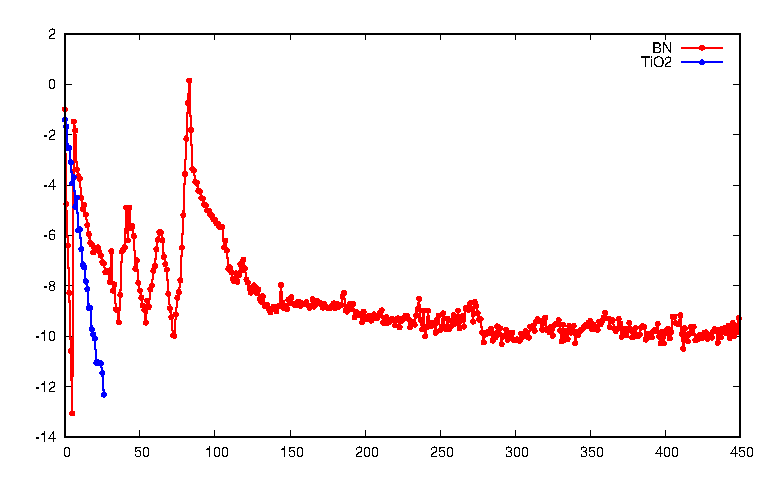
\includegraphics[scale=0.6]{./plots/conv_log.eps}};
%  \node[below=of img1, node distance=0cm, yshift=1cm] {\# iterations};
%  \node[left=of img1, node distance=0cm, rotate=90, anchor=center,yshift=-0.7cm] {ln($\|\nabla E\|$)};
%\end{tikzpicture}
%\caption{Logarithmic plot of convergence vs number of iterations for a conformation of the $r-\text{TiO}_{2}$ nanoparticle. The convergence for a similar DFT calculation on another system (crystalline boron nitride) showing much more numerical instability is shown in red, for comparison purposes.}
%\label{conv}
%\end{figure}

%\tab Finally, our DFT calculations have converged quickly in the majority of cases and have overall exhibited good numerical behaviour (e.g. no radical changes in energy from one iteration to the next, quasi-uniformly decreasing convergence and total energy over the entire length of the calculation).
%Figure \ref{conv} shows the convergence of a DFT calculation made on a conformation the 72-atom $r-\text{TiO}_2$ nanocrystal (in blue).
%As is clearly visible, the convergence steadily decreases as the calculation progresses thereby implying that the changes being made to the computed energy value are getting smaller with each iteration of the DFT energy calculation routine.
%This behaviour suggests that the calculation does not exhibit significant numerical error and that the result it outputs is very likely physical.

\subsection{Comparing classical MD with KS DFT}

\tab For each nanoparticle, we compare the classically evaluated energy of every configuration with the energy obtained through a DFT calculation for that some configuration. 
We plot our results in figures 2-6; a $y=x$ line was added to every plot to give a better appreciation of the level of correlation between classical and DFT data sets.
This allows us to gauge the accuracy of MA forcefield; if the classical and quantum mechanical results are well correlated, then the purely classical representation of the forces in the nanoparticles is sufficiently accurate to discriminate between slight variations in a given system's configuration in a meaningful way and can therefore be used to simulate this system nanoparticles instead of DFT, which is much more computationally expensive.

\begin{figure}[htb]
\begin{tikzpicture}
  \node (img1)  {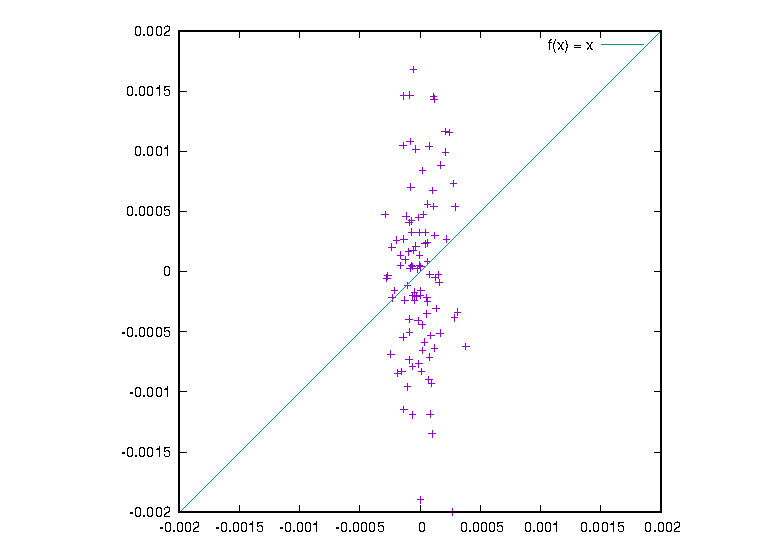
\includegraphics[scale=0.6]{./plots/rutile_72_scaled}};
  \node[below=of img1, node distance=0cm, yshift=1cm] {$E_{\text{classical}} - \bar{E}_{\text{classical}}$ (Ha/atom)};
  \node[left=of img1, node distance=0cm, rotate=90, anchor=center,yshift=-0.7cm] {$E_{\text{DFT}} - \bar{E}_{\text{DFT}}$ (Ha/atom)};
\end{tikzpicture}
\caption{DFT energy vs. classical energy (both shifted down by their average value) for 101 conformations of an $r-\text{TiO}_2$ lattice with 72 atoms.}
\label{rutile72}
\end{figure}

\begin{figure}[htb]
\begin{tikzpicture}
  \node (img1)  {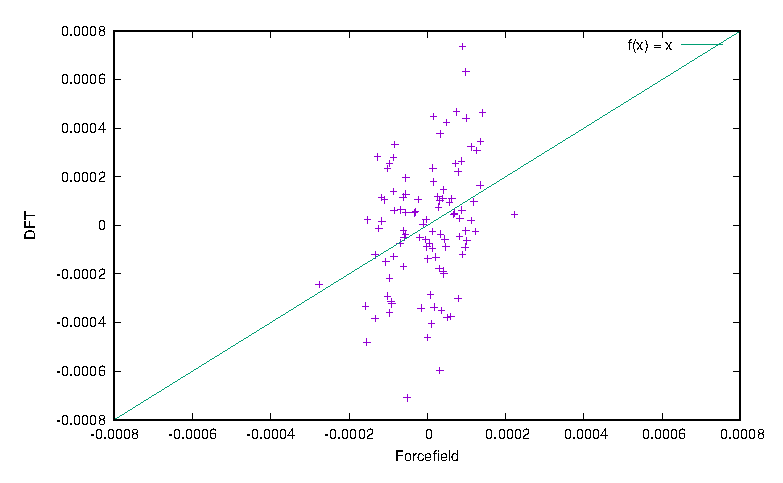
\includegraphics[scale=0.6]{./plots/nnp_198_scaled}};
  \node[below=of img1, node distance=0cm, yshift=1cm] {$E_{\text{classical}} - \bar{E}_{\text{classical}}$ (Ha/atom)};
  \node[left=of img1, node distance=0cm, rotate=90, anchor=center,yshift=-0.7cm] {$E_{\text{DFT}} - \bar{E}_{\text{DFT}}$ (Ha/atom)};
\end{tikzpicture}
\caption{DFT energy vs. classical energy (both shifted down by their average value) for 101 conformations of an $a-\text{TiO}_2$ nanoparticle with 198 atoms.}
\label{nnp_198}
\end{figure}

\tab Comparing the energies obtained using classical MD and those calculated using DFT reveals that a description of the forces inside an $a-\text{TiO}_2$ nanoparticle using only the two-body MA potential is not precise enough to yield an accurate representation of its PES.
Indeed, plotting the energies yielded by both calculation methods reveals that DFT calculation methods are much more sensitive to a change in a given nanoparticle's atomic configuration than classical methods.

\begin{figure}[htb]
\begin{tikzpicture}
  \node (img1)  {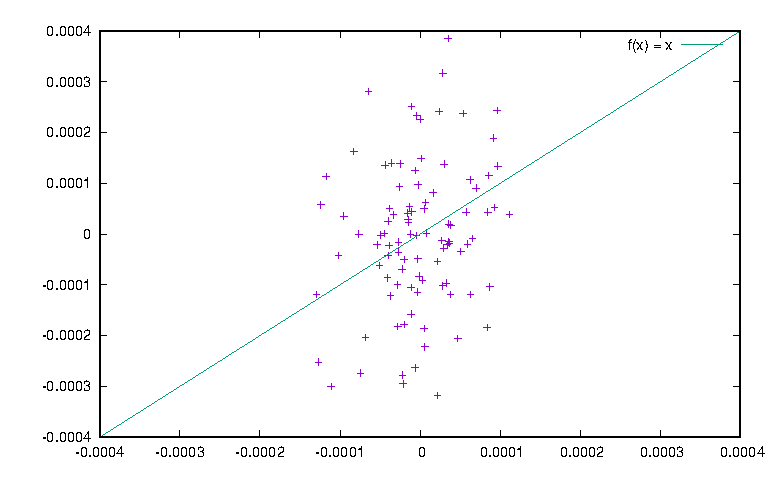
\includegraphics[scale=0.6]{./plots/nnp_390_scaled}};
  \node[below=of img1, node distance=0cm, yshift=1cm] {$E_{\text{classical}} - \bar{E}_{\text{classical}}$ (Ha/atom)};
  \node[left=of img1, node distance=0cm, rotate=90, anchor=center,yshift=-0.7cm] {$E_{\text{DFT}} - \bar{E}_{\text{DFT}}$ (Ha/atom)};
\end{tikzpicture}
\caption{DFT energy vs. classical energy (both shifted down by their average value) for 101 conformations of an $a-\text{TiO}_2$ nanoparticle with 390 atoms.}
\label{nnp_390}
\end{figure}

\tab The system for which this is the most obvious is the 768 atom nanoparticle, for which all classically evaluated energies lie within $\sim 10^{-4}\,\text{Ha}$ of each other, while the energies obtained usinq quantum mechanical methods vary by $\sim 10^{-1}\,\text{Ha}$.
One can get a sense of how dramatic this disparity between the ranges of of both data sets by examining figure \ref{nnp_768}: when plotting the DFT and classical data on the same scale, the classical energy values almost all lie on the same vertical line and thus appear to all be identical. 
While this effect is most dramatic for the 768 atom system, every other nanoparticle on which we ran similar calculations exhibit significant clustering of the energies obtained using the MA potential about their mean value, while their DFT energies spread out over a much larger interval.

\begin{figure}[htb]
\begin{tikzpicture}
  \node (img1)  {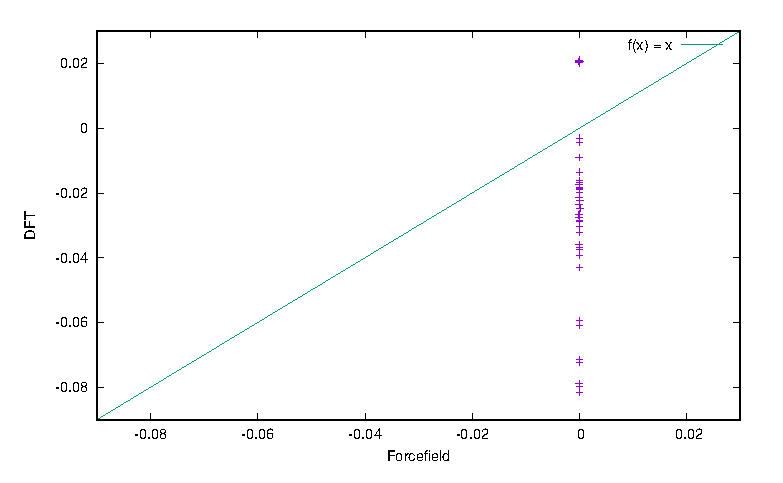
\includegraphics[scale=0.6]{./plots/nnp_768_fully_scaled}};
  \node[below=of img1, node distance=0cm, yshift=1cm] {$E_{\text{classical}} - \bar{E}_{\text{classical}}$ (Ha/atom)};
  \node[left=of img1, node distance=0cm, rotate=90, anchor=center,yshift=-0.7cm] {$E_{\text{DFT}} - \bar{E}_{\text{DFT}}$ (Ha/atom)};
\end{tikzpicture}
\caption{DFT energy vs. classical energy (both shifted down by their average value) for 101 conformations of an $a-\text{TiO}_2$ nanoparticle with 768 atoms.}
\label{nnp_768}
\end{figure}
  
\tab All four systems we ran these calculations on exhibit weak correlation between the DFT-calculated energy values and the energies obtained using the MA potential. 
Even more surprisingly, we find that the two sets of energy values of the different conformations of the rutile lattice were even less correlated than the ones obtained from the amorphous nanoparticles. 
As can be seen in table \ref{stats}, our simulated rutile lattice yielded the lowest value of $\rho$ of all the systems we studied.

%\begin{figure}[htb]
%\begin{tikzpicture}
%  \node (img1)  {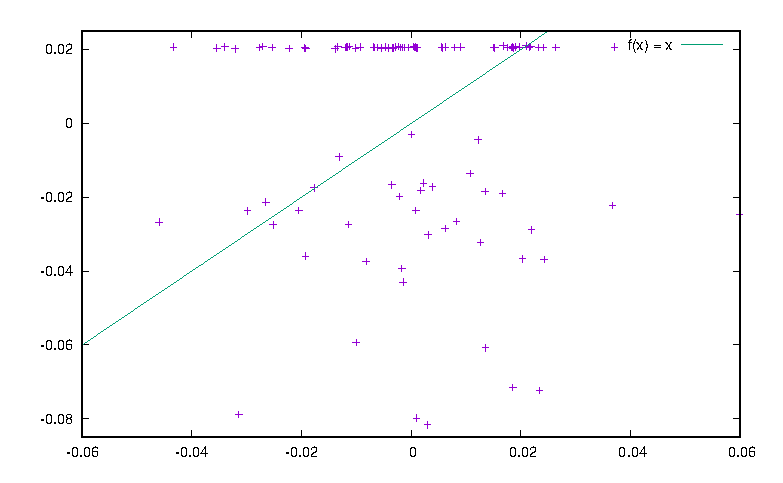
\includegraphics[scale=0.6]{./plots/nnp_768_dilated}};
%  \node[below=of img1, node distance=0cm, yshift=1cm] {$500\cdot (E_{\text{classical} - \bar{E}_{\text{classical}})}$ (Ha/atom)};
%  \node[left=of img1, node distance=0cm, rotate=90, anchor=center,yshift=-0.7cm] {$E_{\text{DFT}} - \bar{E}_{\text{DFT}}$ (Ha/atom)};
%\end{tikzpicture}
%\caption{Dilated version of figure \ref{nnp_768}.}
%\label{nnp_768d}
%\end{figure}

In light of this extremely low correlation, we cannot consider our simulated $r-\text{TiO}_2$ lattice a reference system.
This unexpectedly poor correlation between these two sets of energy values also questions the accuracy of our DFT results, which have been our accuracy benchmark throughout this paper.

\tab Assuming that our DFT calculations are indeed accurate, this lack of correlation between the energies obtained from $r-\text{TiO}_2$ is not overly problematic; it could simply suggests that a purely classical two-body description of atomic interactions in $\text{TiO}_2$ in the amorphous or rutile phase is not sufficiently accurate to keep track of small changes in the system's configuration.
Moreover the small RMSE values we get for all systems (except the 768-atom nanoparticle) and the fact that all classically obtained energies for a given system are very close to each other suggest that they are still physically sound at a less precise level of analysis.
If both sets of energy values for each system varied over intervals of similar sizes and yet remained as uncorrelated as we have observed them to be, then the validity of trying to describe $\text{TiO}_2$ using only the MA potential would be seriously questioned.
However this is not the case; for every system all energies computed classically differ very little.
This is consistent with the fact that the atomic configurations from which such energies are computed were obtained from segments of our MD simulations where the system was already at equilibrium with its environment (i.e. the thermal bath) and thus did not vary greatly either.
It is therefore reassuring to see that, within our classical MD simulation, snapshots which have similar structures are also found to have close energy values. 
The contrast between the highly clustered classical values and the much more spread out quantum values could therefore suggest that the quantum description of $\text{TiO}_2$ is much more sensitive to the system's conformational changes while using the MA potential cannot meaningfully register such changes yet still provides an internally consistent and physically viable picture of the system.
This is further suggested by other works which only used the MA potential to model $\text{TiO}_2$ (in both amorphous and crystalline states) and have successfully reproduced a number of experimental findings on the local atomic structure of the systems being considered\cite{vvh1,vvh2,fichtorn}.
Interpreting our findings in this light would lead us to the conclusion that while the MA picture is sufficient to meaningfully describe some of titania's structural properties, one would still need DFT to properly describe its electronic structure and its related characteristics (e.g. magnetic behaviour, dielectric constant, etc.). 

\begin{table*}[]
\begin{tabular}{c|c|c|c|c}
System & $a-\text{TiO}_2$ (198 atoms) & $a-\text{TiO}_2$ (390 atoms) & $a-\text{TiO}_2$ (768 atoms)  & $r-\text{TiO}_2$ (72 atoms) \\ \hline
$\rho$ & 0.3066474                    & 0.3497706                    & -0.0496755                   & 0.0141203                   \\
RMSE   & 0.0486056                    & 0.0628487                    & 22.21090                       & 0.0518275                   \\
\end{tabular}
\label{stats}
\caption{Pearson correlation coefficient $\rho$ and RMSE between the energy values obtained through DFT and those obtained using the two-body MA potential on various configurations of different systems.}
\end{table*}

%\tab As stated in the previous paragraph, it could also be possible that the results we obtained $\textit{via}$ DFT are inaccurate.
%While this is unlikely (see previous subsection), a few different factors could be responsible for corrupting our DFT data.
%A possible explanation is that we obtained our classical energy values from an MD simulation with $T=300\,$K while our DFT routine calculates the ground state energy of a system at $T=0\,$K.
%This discrepancy between the assumptions made by both calculation methods could explain why our energy values for our simulated $r-\text{TiO}_2$ nanostructures are so weakly correlated.
%This is unlikely however, seeing as the overwhelming majority of the system's electrons would remain in their ground state at $T=300\,$K, thus leaving the system's PES unchanged.

\tab As we have seen, there is a serious discrepancy between the PES predicted by the MA force-field and that predicted by DFT.
While this is hardly surprising, the difference between both models' respective PESs raises some interesting problems when trying to directly compare the energy of a particular arrangement of atoms given by both methods. 
We obtained our structures from MD simulations that used the MA potential and allowed the atomic configurations of our different systems to equilibrate with the thermal bath of each run.
We are therefore running all of our energy calculations on conformations sampled from the region surrounding a local minimum of the MA PES of our different systems, which implies that these conformations' MA energies will all be very close to one another ($|\nabla^N V_{\text{classical}}|\sim 0$ near a minimum of the classical PES).
This will not be the case for the energies we obtain using DFT because MA-obtained atomic configurations do not lie near a local minimum of the PES predicted by DFT.
We can therefore expect $|\nabla^N V_{\text{DFT}}|$ to be non-negligible for those conformations, thus leading to large differences in DFT-computed energies from one configuration to the next.
This is exactly what we observe for both crystalline and amorphous titania.
Figure 5 shows a schematic explanation of how this disagreement between the two PESs yields the clustered values we observe in our MA energy sets and the disperse values characteristic of our DFT energy sets.
For simplicity, both the $3N$-dimensional PESs obtained are represented as unidimensional and are assumed to be harmonic with local minima located near one another (i.e. functions of the form of $V(x) = k\cdot (x-x_0)^2$).
As the figure clearly shows, two qualitatively similar PESs with slightly different topologies can yield energy values that are poorly correlated uncorrelated.

\begin{figure*}
\centering
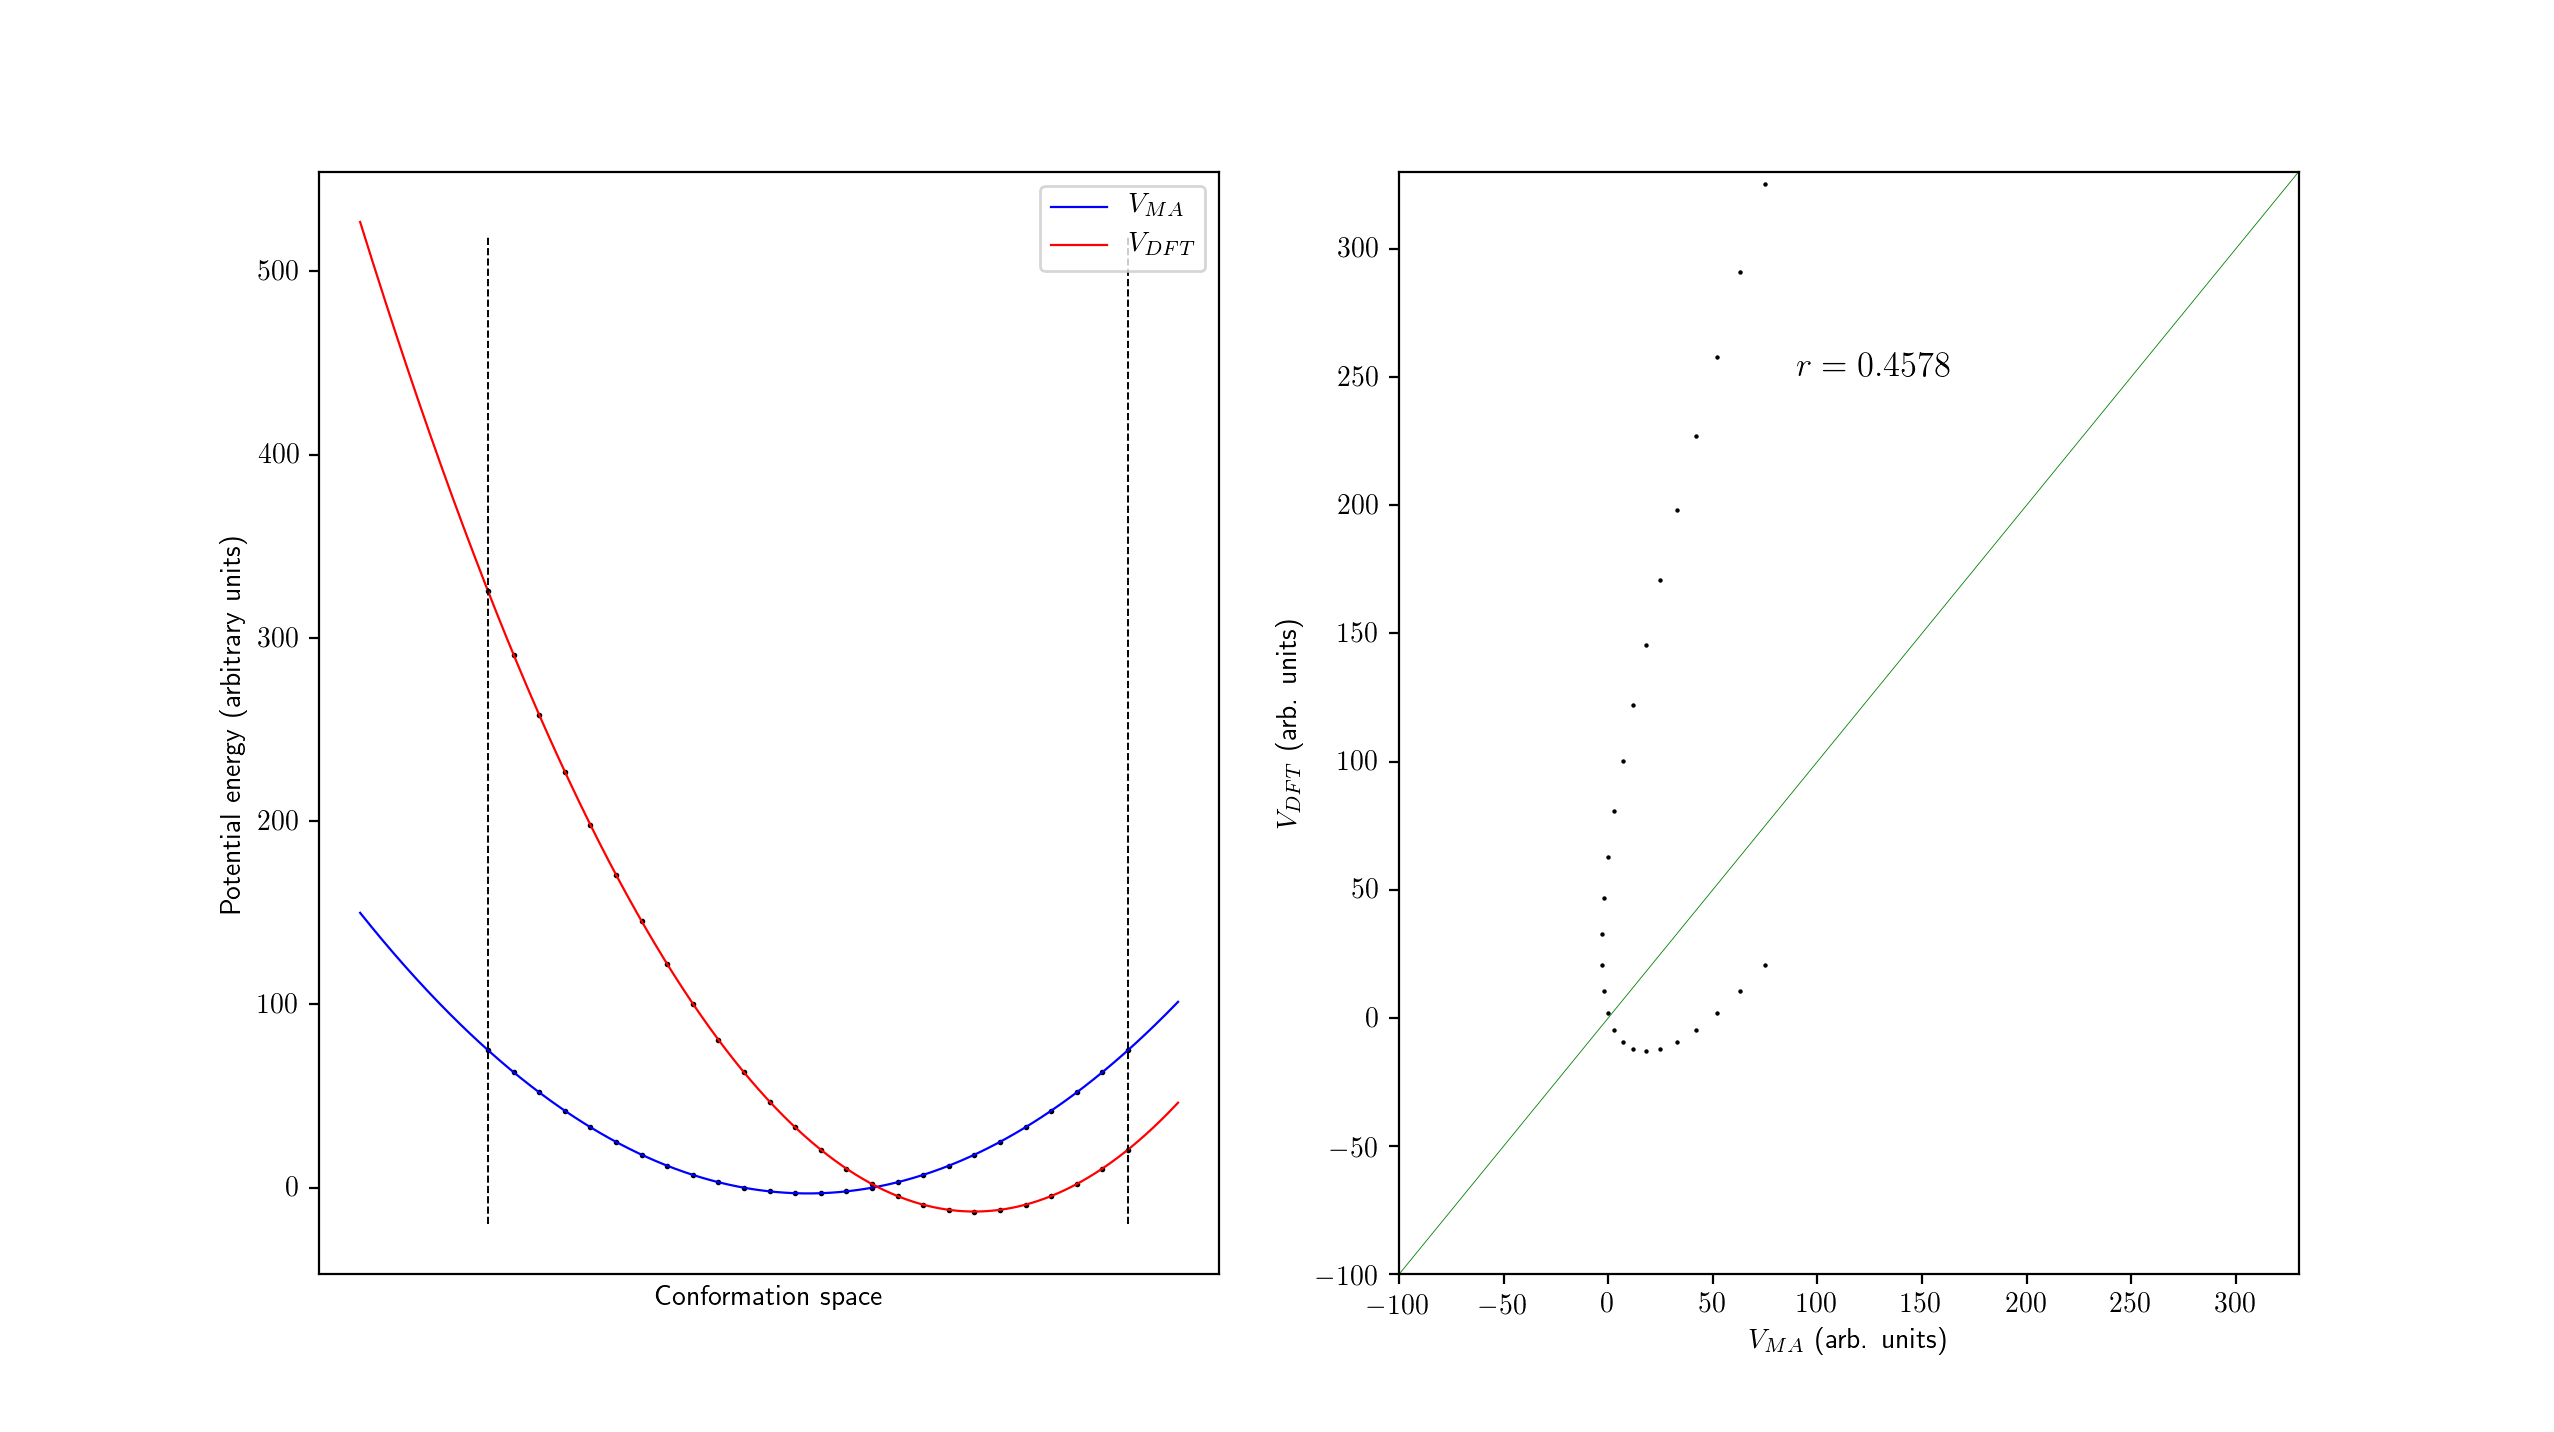
\includegraphics[scale=0.5]{./plots/pseudo-PES}
\label{pes}
\caption{Schematic representation of the problems arising from direct comparison of energy values yielded by differing PESs. In the left-hand plot both PESs are assumed to be 1-dimensional (instead of depending on the $3N$ position variables of the system's $N$ atoms). We can see how conformations (black dots) sampled near the minimum of the MA PES (blue curve) are much more spread out in energy when projected on the PES obtained using DFT (red curve), yielding a similar comparison to the one drawn by our data. The right-hand scatter plot presents the energies obtained from both PESs in the same way we plotted the actual energy values obtained from our calculations, and $r$ denotes the Pearson correlation coefficient between both sets of sampled energies.}
\end{figure*}

\tab Our method of directly comparing the energies of individual conformations is therefore overly naive.
A better way to compare the accuracy of DFT with the MA force-field would be to generate structures using both methods instead of comparing the energies of structures obtained solely using classical MD using the MA potential.
One could then compare the structural properties (e.g. density, average bond lengths, etc.) of both sets of configurations to their experimentally observed values and determine which method yields the most precise predictions.
A sketch-map\cite{sketch-map} algorithm could also be used to judge the similarity between DFT-obtained structures and those generted by the MA potential.
The proportion of conformations obtained through both methods that are alike would give us another indicator of the level of agreement between both models. 

\tab Surface effects could also be an important factor responsible for the uncorrelatedness of our $a-\text{TiO}_2$ energy values.  
As previously stated, the MA potential was developed to reproduce the bulk structures of $\text{TiO}_2$ in its various crystalline forms; the potential was developed by simulating nanocrystals ranging from 384 atoms to 576 atoms in size and the bulk properties of the different crystalline polytypes of titania were used to fix its energy parameters\cite{MA_og}.
Knowing that the surface sites of a $\text{TiO}_2$ nanoparticle (crystalline or amorphous) have significantly different atomic and electronic structures as bulk sites\cite{vvh1,realistic_nnp,vvh2}, it is easy to see how a model built to simulate systems containing mainly bulk sites can reach erroneous results when trying reproduce a nanoparticle with a significant portion of its atoms on the surface.
It is probable that conducting a similar study on set of larger $a-\text{TiO}_2$ nanoparticles would yield better correlated classical and DFT energy values.
Unfortunately, running DFT single-point energy calculations on larger nanoparticles might prove to be prohibitively computationally expensive without optimising the DFT calculation scheme to handle systems with many atoms ($>1000$ atoms).

\tab Computational expense being one of DFT's main drawbacks, a number of optimisation schemes have been proposed over the years to reduce both the amount of memory and the time necessary to run calculations on large systems ($\sim 1000$ atoms).
Among them, the absolutely localised molecular orbitals\cite{almo} (ALMO) method partitions the simulated system into small fragments (usually the individual atoms or molecules that compose it) and runs traditional DFT on each fragment in parallel.
This has the advantage of having a runtime that scales linearly with the number of fragments for large systems, while traditional DFT calculation runtimes scale cubically with the number of atoms being simulated.
Seeing as ALMO DFT makes a number of large DFT calculations much more feasible, it would allow us to conduct a similar study on larger nanoparticles (with more bulk sites) which could potentially yield better correlated classical and DFT values.
This could furthermore enable us to run simulations of nanoparticles with sizes closer to those of $a-\text{TiO}_2$ nanoparticles used in most practical applications ($\sim 4\,$nm\cite{realistic_nnp}) and therefore give us a better appreciation of how the MA potential performs on systems it is better adapted to model.

\tab Another way to run similar calculations on larger $\text{TiO}_2$ nanoparticles would be use smaller basis sets.
While the basis set we used to describe oxygen's electronic distribution (DZVP) cannot be further reduced without removing a polarisation function (which is crucial to adequately describe chemical bonding), the basis set we used for Ti explicitly describes the electrons in its three highest occupied subshells ($3p,\,3d,$ and $4s$).
Knowing that we can safely assume that titanum's six $3p$ elctrons have negligible impact on bonding in $\text{TiO}_2$\cite{electronic_structure}, we can use a basis set and pseudopotential which treat them as core electrons.
This would significantly reduce the memory cost and computation time of a DFT simulation of any system containing numerous Ti atoms, thus making DFT calculations on large $\text{TiO}_2$ nanoparticles more easily implementable.

\tab Regardless of how well the MA potential describes $r-\text{TiO}_2$, the data we obtained from modeling amorphous systems unequivocally indicates that the picture of $\text{TiO}_2$ provided by the MA potential is not consistent with DFT's description of the material.

%\tab Another possible explanation for the uncorrelatedness of the $r-\text{TiO}_2$ energy sets is our simulated lattice's small size.
%As previously stated, the MA potential was developed to reproduce the bulk structures of $\text{TiO}_2$ in its various crystalline forms; the potential was developed by simulating nanocrystals ranging from 384 atoms to 576 atoms in size and the bulk properties of the different crystalline polytypes of titania were used to fix its energy parameters.
%Knowing that the surface sites of a $\text{TiO}_2$ nanoparticle (crystalline or amorphous) have significantly different atomic and electronic structures as bulk sites\cite{vvh1,realistic_nnp,vvh2}, it is easy to see how a model built to simulate systems containing mainly bulk sites can reach erroneous results when trying reproduce a nanoparticle with a significant portion of its atoms on the surface.
%It is probable that a classical MD simulation of a larger $r-\text{TiO}_2$ lattice would yield a better set of reference conformation and energy values.
%Unfortunately, running DFT single-point energy calculations on larger nanoparticles might prove to be prohibitively computationally expensive without optimising the DFT calculation scheme to handle systems with many atoms ($>1000$ atoms).
%Regardless of how well the MA potential describes $r-\text{TiO}_2$, the data we obtained from modeling amorphous systems unequivocally indicates that the picture of $\text{TiO}_2$ provided by the MA potential is not always consistent with the DFT's description of the material.
 

%\begin{table*}[]
%\begin{tabular}{c|c|c|c|c|c}
%System & $a-\text{TiO}_2$ (198 atoms) & $a-\text{TiO}_2$ (390 atoms) & $a-\text{TiO}_2$ (768 atoms) & $a-\text{TiO}_2$ (1842 atoms) & $r-\text{TiO}_2$ (72 atoms) \\ \hline
%$\rho$ & 0.3066474                    & 0.3497706                    & -0.0496755                   & TBC                           & 0.0141203                   \\
%RMSE   & 0.0486056                    & 0.0628487                    & 22.21090                     & TBC                           & 0.0518275                   \\
%\end{tabular}
%\label{stats}
%\caption{Pearson correlation coefficient $\rho$ and RMSE between the energy values obtained through DFT and those obtained using the two-body MA potential on various configurations of different systems.}
%\end{table*}

%\subsection{Comparing ALMO DFT with KS DFT}
 
%[FURTHER DISCUSSION: unshifted DFT values are ~500times larger than unshifted classical values rescale shifted energy values by dividing by average E?] 
 
\section*{Conclusion}

%\tab This paper's main objective was to quantify the accuracy of a simulation of amorphous titania nanoparticles using classical formalism.
%Using a set of common atomic configuration, we compared energy values obtained $\textit{via}$ a DFT calculation and those obtained using the classical MA potential, for $a-\text{TiO}_2$ nanoparticles of different sizes.
%All of the systems we simulated showed weak correlation between the classical and DFT energy values.

\tab Our comparison of the energy values we obtained through DFT and those calculated with the classical MA potential, on common sets of conformations of various $\text{TiO}_2$ nanoparticles has consistently revealed that these two data sets are weakly correlated.
These results imply that the PES of a small $a-\text{TiO}_2$ predicted by the MA force-field is significantly different from the one produced by KS DFT.
Having established our DFT results to be more accurate than the ones yielded by the MA potential, we can safely assume that the MA potential does not faithfully reproduce the PES of small titania nanoparticles.
This holding true even for the set of energies obtained from a system which we believed to be well-described by both methods -- a 72-atom rutile lattice -- raises some questions about the validity of our methods and calls for further research into this topic.
The observed discrepancy between the PESs yielded by both models invalidates our approach of comparing the energies of different atomic configurations directly to one another; it fails to account for the change in topology between both energy surfaces thus making both methods appear more disparate than they might truly be.

%\begin{itemize}
%\item Are surface sites responsible for the disagreement between our energy values for $r-\text{TiO}_2$?
%\item How necessary is the additional detail provided by DFT calculations to derive meaningful results from simulations of $\text{TiO}_2$ nanoparticles? 
%\end{itemize}
%These problems left unsolved call for further research into this topic; we examine certain possible ways in which the answers to the question posed here can be further elucidated.

%\tab Assuming that DFT calculations are necessary to properly sample from an $a-\text{TiO}_2$ nanoparticle's PES, we are now faced with the problem posed by the computing power necessary to run such calculations on large systems (i.e. nanoparticles containing more than $\sim\,$1000 atoms).

\tab Conducting classical and DFT simulations on larger nanoparticles could also provide further insight,since the structure and properties of large nanoparticles are less impacted by their surface sites than smaller nanoparticles\cite{realistic_nnp}.
This motivates the development of cheaper, more scalable DFT schemes.  
Being able to carry out such calculations on large systems could eventually allow for full MD simulations of nanoparticulate titania using DFT.
This would give researchers the means to generate atomic structures of $\text{TiO}_2$ nanoparticles from first principles only. 
Comparing these $\textit{ab-initio}$ structures' properties (e.g. density, bulk/surface coordination number, average bond length) to those of structures obtained through experiment or using classical potentials might also offer insight on how well-suited both simulations methods are to describing such systems.
Implementations of DFT that are optimised for large systems could also be used to study the size dependence of many of nanoparticulate titania's properties and to examine whether our current models can adequately account for them. 

\tab This work therefore raises more questions than it answers.
Fortunately, the problems posed by our results leave us with a clear sense of what needs to be done to further elucidate the level of accuracy of classical MD simulations of amorphous titania.
The main axes of future research we propose is the modelisation of larger, more practically relevant nanoparticles and the use of linear scaling DFT routines to simulate such nanoparticles from first principles.
%\tab Having observed that DFT calculations are necessary to properly sample from an $a-\text{TiO}_2$ nanoparticle's PES, we are now faced with the problem posed by the computing power necessary to run such calculations on large systems (i.e. nanoparticles containing more than $\sim\,$1000 atoms).
%Seeing as computational expense is one of DFT's main drawbacks, a number of optimisation schemes have been proposed over the years to reduce both the amount of memory and the time necessary to run such calculations.
%Among them, we focus our attention to the absolutely localised molecular orbitals (ALMO) method which partitions the system being simulated into smaller fragments (usually these are the individual atoms or molecules that compose it) and runs traditional DFT on each fragment in parallel.
%This has the advantage of having a runtime that scales linearly with the number of fragments for large systems.
%Seeing as ALMO DFT makes a number of large DFT calculations much more feasible, we decide to test its accuracy on our various $a-\text{TiO}_2$ nanoparticles.
%As before, we evaluate the accuracy of the ALMO DFT method by comparing the energy it outputs for a given configuration of a nanoparticle with the energy obtained through classical DFT.  

%\textbf{Supporting Information}
%Calculated radial distribution functions of liquid water, comparison of timing benchmarks for the DZVP and TZV2P basis sets, timing benchmarks for systems containing 32,768 water molecules, timing benchmarks for the Kohn-Sham matrix build. This material is available free of charge via the Internet at http://pubs.acs.org.

%\textbf{Acknowledgments.} The research was funded by the Natural Sciences and Engineering Research Council of Canada through the Discovery Grant. The authors are grateful to Compute Canada and McGill HPC Centre for computer time.

\bibliography{tio2_nnp}

\end{document}
